% Generated by Sphinx.
\def\sphinxdocclass{report}
\documentclass[a4paper,12pt,english]{sphinxmanual}
\usepackage[utf8]{inputenc}
\DeclareUnicodeCharacter{00A0}{\nobreakspace}
\usepackage[T1]{fontenc}
\usepackage{babel}
\usepackage{times}
\usepackage[Bjarne]{fncychap}
\usepackage{longtable}
\usepackage{sphinx}
\usepackage{multirow}


\title{VIS Documentation}
\date{July 03, 2012}
\release{0.1}
\author{Sami-Matias Niemi}
\newcommand{\sphinxlogo}{}
\renewcommand{\releasename}{Release}
\makeindex

\makeatletter
\def\PYG@reset{\let\PYG@it=\relax \let\PYG@bf=\relax%
    \let\PYG@ul=\relax \let\PYG@tc=\relax%
    \let\PYG@bc=\relax \let\PYG@ff=\relax}
\def\PYG@tok#1{\csname PYG@tok@#1\endcsname}
\def\PYG@toks#1+{\ifx\relax#1\empty\else%
    \PYG@tok{#1}\expandafter\PYG@toks\fi}
\def\PYG@do#1{\PYG@bc{\PYG@tc{\PYG@ul{%
    \PYG@it{\PYG@bf{\PYG@ff{#1}}}}}}}
\def\PYG#1#2{\PYG@reset\PYG@toks#1+\relax+\PYG@do{#2}}

\def\PYG@tok@gd{\def\PYG@tc##1{\textcolor[rgb]{0.63,0.00,0.00}{##1}}}
\def\PYG@tok@gu{\let\PYG@bf=\textbf\def\PYG@tc##1{\textcolor[rgb]{0.50,0.00,0.50}{##1}}}
\def\PYG@tok@gt{\def\PYG@tc##1{\textcolor[rgb]{0.00,0.25,0.82}{##1}}}
\def\PYG@tok@gs{\let\PYG@bf=\textbf}
\def\PYG@tok@gr{\def\PYG@tc##1{\textcolor[rgb]{1.00,0.00,0.00}{##1}}}
\def\PYG@tok@cm{\let\PYG@it=\textit\def\PYG@tc##1{\textcolor[rgb]{0.25,0.50,0.56}{##1}}}
\def\PYG@tok@vg{\def\PYG@tc##1{\textcolor[rgb]{0.73,0.38,0.84}{##1}}}
\def\PYG@tok@m{\def\PYG@tc##1{\textcolor[rgb]{0.13,0.50,0.31}{##1}}}
\def\PYG@tok@mh{\def\PYG@tc##1{\textcolor[rgb]{0.13,0.50,0.31}{##1}}}
\def\PYG@tok@cs{\def\PYG@tc##1{\textcolor[rgb]{0.25,0.50,0.56}{##1}}\def\PYG@bc##1{\colorbox[rgb]{1.00,0.94,0.94}{##1}}}
\def\PYG@tok@ge{\let\PYG@it=\textit}
\def\PYG@tok@vc{\def\PYG@tc##1{\textcolor[rgb]{0.73,0.38,0.84}{##1}}}
\def\PYG@tok@il{\def\PYG@tc##1{\textcolor[rgb]{0.13,0.50,0.31}{##1}}}
\def\PYG@tok@go{\def\PYG@tc##1{\textcolor[rgb]{0.19,0.19,0.19}{##1}}}
\def\PYG@tok@cp{\def\PYG@tc##1{\textcolor[rgb]{0.00,0.44,0.13}{##1}}}
\def\PYG@tok@gi{\def\PYG@tc##1{\textcolor[rgb]{0.00,0.63,0.00}{##1}}}
\def\PYG@tok@gh{\let\PYG@bf=\textbf\def\PYG@tc##1{\textcolor[rgb]{0.00,0.00,0.50}{##1}}}
\def\PYG@tok@ni{\let\PYG@bf=\textbf\def\PYG@tc##1{\textcolor[rgb]{0.84,0.33,0.22}{##1}}}
\def\PYG@tok@nl{\let\PYG@bf=\textbf\def\PYG@tc##1{\textcolor[rgb]{0.00,0.13,0.44}{##1}}}
\def\PYG@tok@nn{\let\PYG@bf=\textbf\def\PYG@tc##1{\textcolor[rgb]{0.05,0.52,0.71}{##1}}}
\def\PYG@tok@no{\def\PYG@tc##1{\textcolor[rgb]{0.38,0.68,0.84}{##1}}}
\def\PYG@tok@na{\def\PYG@tc##1{\textcolor[rgb]{0.25,0.44,0.63}{##1}}}
\def\PYG@tok@nb{\def\PYG@tc##1{\textcolor[rgb]{0.00,0.44,0.13}{##1}}}
\def\PYG@tok@nc{\let\PYG@bf=\textbf\def\PYG@tc##1{\textcolor[rgb]{0.05,0.52,0.71}{##1}}}
\def\PYG@tok@nd{\let\PYG@bf=\textbf\def\PYG@tc##1{\textcolor[rgb]{0.33,0.33,0.33}{##1}}}
\def\PYG@tok@ne{\def\PYG@tc##1{\textcolor[rgb]{0.00,0.44,0.13}{##1}}}
\def\PYG@tok@nf{\def\PYG@tc##1{\textcolor[rgb]{0.02,0.16,0.49}{##1}}}
\def\PYG@tok@si{\let\PYG@it=\textit\def\PYG@tc##1{\textcolor[rgb]{0.44,0.63,0.82}{##1}}}
\def\PYG@tok@s2{\def\PYG@tc##1{\textcolor[rgb]{0.25,0.44,0.63}{##1}}}
\def\PYG@tok@vi{\def\PYG@tc##1{\textcolor[rgb]{0.73,0.38,0.84}{##1}}}
\def\PYG@tok@nt{\let\PYG@bf=\textbf\def\PYG@tc##1{\textcolor[rgb]{0.02,0.16,0.45}{##1}}}
\def\PYG@tok@nv{\def\PYG@tc##1{\textcolor[rgb]{0.73,0.38,0.84}{##1}}}
\def\PYG@tok@s1{\def\PYG@tc##1{\textcolor[rgb]{0.25,0.44,0.63}{##1}}}
\def\PYG@tok@gp{\let\PYG@bf=\textbf\def\PYG@tc##1{\textcolor[rgb]{0.78,0.36,0.04}{##1}}}
\def\PYG@tok@sh{\def\PYG@tc##1{\textcolor[rgb]{0.25,0.44,0.63}{##1}}}
\def\PYG@tok@ow{\let\PYG@bf=\textbf\def\PYG@tc##1{\textcolor[rgb]{0.00,0.44,0.13}{##1}}}
\def\PYG@tok@sx{\def\PYG@tc##1{\textcolor[rgb]{0.78,0.36,0.04}{##1}}}
\def\PYG@tok@bp{\def\PYG@tc##1{\textcolor[rgb]{0.00,0.44,0.13}{##1}}}
\def\PYG@tok@c1{\let\PYG@it=\textit\def\PYG@tc##1{\textcolor[rgb]{0.25,0.50,0.56}{##1}}}
\def\PYG@tok@kc{\let\PYG@bf=\textbf\def\PYG@tc##1{\textcolor[rgb]{0.00,0.44,0.13}{##1}}}
\def\PYG@tok@c{\let\PYG@it=\textit\def\PYG@tc##1{\textcolor[rgb]{0.25,0.50,0.56}{##1}}}
\def\PYG@tok@mf{\def\PYG@tc##1{\textcolor[rgb]{0.13,0.50,0.31}{##1}}}
\def\PYG@tok@err{\def\PYG@bc##1{\fcolorbox[rgb]{1.00,0.00,0.00}{1,1,1}{##1}}}
\def\PYG@tok@kd{\let\PYG@bf=\textbf\def\PYG@tc##1{\textcolor[rgb]{0.00,0.44,0.13}{##1}}}
\def\PYG@tok@ss{\def\PYG@tc##1{\textcolor[rgb]{0.32,0.47,0.09}{##1}}}
\def\PYG@tok@sr{\def\PYG@tc##1{\textcolor[rgb]{0.14,0.33,0.53}{##1}}}
\def\PYG@tok@mo{\def\PYG@tc##1{\textcolor[rgb]{0.13,0.50,0.31}{##1}}}
\def\PYG@tok@mi{\def\PYG@tc##1{\textcolor[rgb]{0.13,0.50,0.31}{##1}}}
\def\PYG@tok@kn{\let\PYG@bf=\textbf\def\PYG@tc##1{\textcolor[rgb]{0.00,0.44,0.13}{##1}}}
\def\PYG@tok@o{\def\PYG@tc##1{\textcolor[rgb]{0.40,0.40,0.40}{##1}}}
\def\PYG@tok@kr{\let\PYG@bf=\textbf\def\PYG@tc##1{\textcolor[rgb]{0.00,0.44,0.13}{##1}}}
\def\PYG@tok@s{\def\PYG@tc##1{\textcolor[rgb]{0.25,0.44,0.63}{##1}}}
\def\PYG@tok@kp{\def\PYG@tc##1{\textcolor[rgb]{0.00,0.44,0.13}{##1}}}
\def\PYG@tok@w{\def\PYG@tc##1{\textcolor[rgb]{0.73,0.73,0.73}{##1}}}
\def\PYG@tok@kt{\def\PYG@tc##1{\textcolor[rgb]{0.56,0.13,0.00}{##1}}}
\def\PYG@tok@sc{\def\PYG@tc##1{\textcolor[rgb]{0.25,0.44,0.63}{##1}}}
\def\PYG@tok@sb{\def\PYG@tc##1{\textcolor[rgb]{0.25,0.44,0.63}{##1}}}
\def\PYG@tok@k{\let\PYG@bf=\textbf\def\PYG@tc##1{\textcolor[rgb]{0.00,0.44,0.13}{##1}}}
\def\PYG@tok@se{\let\PYG@bf=\textbf\def\PYG@tc##1{\textcolor[rgb]{0.25,0.44,0.63}{##1}}}
\def\PYG@tok@sd{\let\PYG@it=\textit\def\PYG@tc##1{\textcolor[rgb]{0.25,0.44,0.63}{##1}}}

\def\PYGZbs{\char`\\}
\def\PYGZus{\char`\_}
\def\PYGZob{\char`\{}
\def\PYGZcb{\char`\}}
\def\PYGZca{\char`\^}
\def\PYGZsh{\char`\#}
\def\PYGZpc{\char`\%}
\def\PYGZdl{\char`\$}
\def\PYGZti{\char`\~}
% for compatibility with earlier versions
\def\PYGZat{@}
\def\PYGZlb{[}
\def\PYGZrb{]}
\makeatother

\begin{document}

\maketitle
\tableofcontents
\phantomsection\label{index::doc}

\begin{quote}\begin{description}
\item[{Author}] \leavevmode
Sami-Matias Niemi

\item[{Contact}] \leavevmode
\href{mailto:smn2@mssl.ucl.ac.uk}{smn2@mssl.ucl.ac.uk}

\item[{version}] \leavevmode
1.0

\end{description}\end{quote}

This Python package provides subpackages and methods related to the visible instrument (VIS) on board
the Euclid satellite. The subpackages include methods to e.g. generate object catalogues, simulate VIS images,
study radiation damage effects and fit new trap species, reduce and analyse data, and to include instrumental
characteristics such as readout noise and CTI to ``pristine'' images generated with e.g. GREAT10 photon
shooting code.


\chapter{Installation}
\label{index:welcome-to-euclid-visible-instrument-vis-documentation}\label{index:installation}
This package contains a mixture of classes and scripts. There is no official or preferred installation
instructions yet. To get most scripts working you should place the path to the root directory of the package
to your PYTHONPATH environment variable. In addition, it is useful to compile the Fortran code available
in the fortran subdirectory with the following command:

\begin{Verbatim}[commandchars=\\\{\}]
f2py -c -m cdm03 cdm03.f90
\end{Verbatim}

and then copy the .so file to the CTI directory. Please note that f2py is available in the NumPy package,
but you still need for example gFortran compiler.


\section{Dependencies}
\label{index:dependencies}
The VIS Python package depends heavily on other Python packages such as NumPy, SciPy, PyFITS, and matplotlib.
Thus it is recommended that on installs a Python distribution like \href{http://www.enthought.com/}{Enthought Python},
which installs all dependencies at once.


\chapter{Creating Object Catalogs}
\label{index:creating-object-catalogs}
The \emph{sources} subpackage contains a script to generate object catalogs with random x and y positions for
stars and galaxies. The magnitudes of stars and galaxies are drawn from input distributions that are
based on observations. As the number of stars depends on the galactic latitude, the script allows
the user to use three different (30, 60, 90 degrees) angles when generating the magnitude distribution for stars
(see the example plot below).
\begin{figure}[htbp]
\centering
\capstart

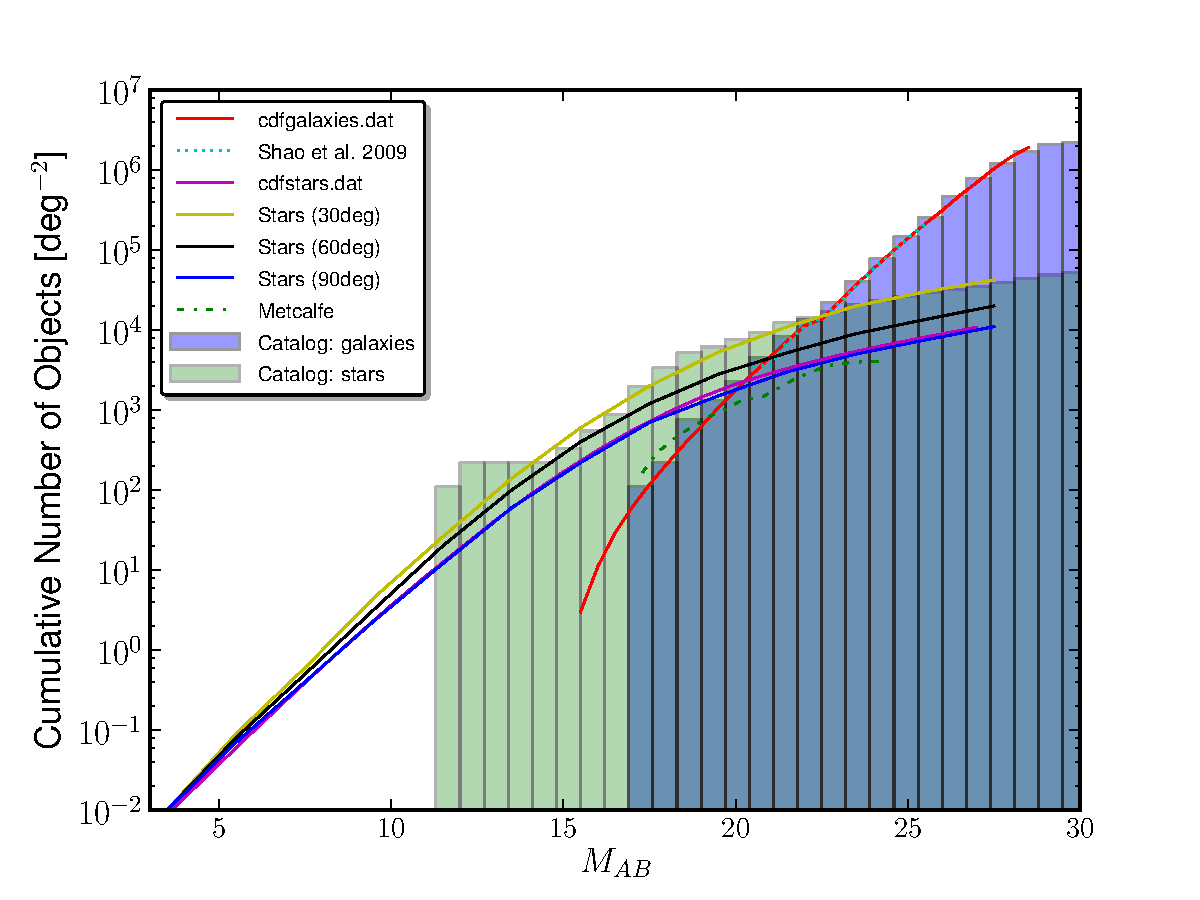
\includegraphics{Distributions.pdf}
\caption{An example showing star and galaxy number counts in a source catalog suitable for VIS simulator.
The solid lines show observations while the histograms show the distributions in the output catalogues.}\end{figure}

For the Python code documentation, please see:
\phantomsection\label{sources:module-sources.createObjectCatalogue}\index{sources.createObjectCatalogue (module)}

\section{Generating Object Catalogue}
\label{sources::doc}\label{sources:generating-object-catalogue}
This simple script can be used to generate an object catalogue that can then be used
as an input for the VIS simulator.

To run:

\begin{Verbatim}[commandchars=\\\{\}]
python createObjectCatalogue.py
\end{Verbatim}

Please note that the script requires files from the data folder. Thus, you should
place the script to an empty directory and either copy or link to the data directory.
\begin{quote}\begin{description}
\item[{requires}] \leavevmode
NumPy

\item[{requires}] \leavevmode
SciPy

\item[{requires}] \leavevmode
matplotlib

\item[{author}] \leavevmode
Sami-Matias Niemi

\item[{contact}] \leavevmode
\href{mailto:smn2@mssl.ucl.ac.uk}{smn2@mssl.ucl.ac.uk}

\end{description}\end{quote}
\index{drawFromCumulativeDistributionFunction() (in module sources.createObjectCatalogue)}

\begin{fulllineitems}
\phantomsection\label{sources:sources.createObjectCatalogue.drawFromCumulativeDistributionFunction}\pysiglinewithargsret{\code{sources.createObjectCatalogue.}\bfcode{drawFromCumulativeDistributionFunction}}{\emph{cpdf}, \emph{x}, \emph{number}}{}
Draw a number of random x values from a cumulative distribution function.
\begin{quote}\begin{description}
\item[{Parameters}] \leavevmode\begin{itemize}
\item {} 
\textbf{cpdf} (\emph{numpy array}) -- cumulative distribution function

\item {} 
\textbf{x} (\emph{numpy array}) -- values of the abscissa

\item {} 
\textbf{number} (\emph{int}) -- number of draws

\end{itemize}

\item[{Returns}] \leavevmode
randomly drawn x value

\item[{Return type}] \leavevmode
ndarray

\end{description}\end{quote}

\end{fulllineitems}

\index{generateCatalog() (in module sources.createObjectCatalogue)}

\begin{fulllineitems}
\phantomsection\label{sources:sources.createObjectCatalogue.generateCatalog}\pysiglinewithargsret{\code{sources.createObjectCatalogue.}\bfcode{generateCatalog}}{\emph{**kwargs}}{}
Generate a catalogue of stars and galaxies that follow
realistic number density functions.
\begin{quote}\begin{description}
\item[{Parameters}] \leavevmode
\textbf{deg} -- galactic latitude, either 30, 60, 90

\end{description}\end{quote}

\end{fulllineitems}

\index{plotDistributionFunction() (in module sources.createObjectCatalogue)}

\begin{fulllineitems}
\phantomsection\label{sources:sources.createObjectCatalogue.plotDistributionFunction}\pysiglinewithargsret{\code{sources.createObjectCatalogue.}\bfcode{plotDistributionFunction}}{\emph{datax}, \emph{datay}, \emph{fitx}, \emph{fity}, \emph{output}}{}
Generates a simple plot showing the observed data points and the fit
that was generated based on these data.

\end{fulllineitems}



\chapter{Generating Simulated Images}
\label{index:generating-simulated-images}
The \emph{simulator} subpackage contains scripts to generate simulated VIS images. Two different methods
of generating mock images is provided. One which takes observed images (say from HST) as an input and
another in which analytical profiles are used for galaxies. The former code is custom made while the
latter relies hevily on IRAF's artdata package and mkobjects task.

The VIS reference simulator is the custom made with real observed galaxies as an input. The IRAF
based simulator can be used, for example, to train algorithms to derive elliptiticy of an object.
For more detailed documentation, please see:


\section{Simulation tools}
\label{simulator:module-simulator.simulator}\label{simulator::doc}\label{simulator:simulation-tools}\index{simulator.simulator (module)}

\subsection{The Euclid Visible Instrument Image Simulator}
\label{simulator:the-euclid-visible-instrument-image-simulator}
This file contains an image simulator for the Euclid VISible instrument.

The approximate sequence of events in the simulator is as follows:
\begin{enumerate}
\item {} 
Read in a configuration file, which defines for example,
detector characteristics (bias, dark and readout noise, gain,
plate scale and pixel scale, oversampling factor, exposure time etc.).

\item {} 
Read in another file containing charge trap definitions (for CTI modelling).

\item {} 
Read in a file defining the cosmic rays (trail lengths and cumulative distributions).

\item {} 
Read in CCD offset information, displace the image, and modify
the output file name to contain the CCD and quadrant information
(note that VIS has a focal plane of 6 x 6 detectors).

\item {} 
Read in source list and determine the number of different object types.

\item {} 
Read in a file which assigns data to a given object index.

\item {} 
Load the PSF model (a single 2D map with a given over sampling or field dependent maps).

\item {} 
Generate a finemap (oversampled image) for each object type. If an object
is a 2D image then calculate the shape tensor to be used for size scaling.
Each type of an object is then placed onto its own finely sampled finemap.

\item {} 
Loop over the number of exposures to co-add and for each object in the object catalog:
\begin{itemize}
\item {} 
determine the number of electrons an object should have by scaling the object's magnitude
with the given zeropoint and exposure time.

\item {} 
determine whether the object lands on to the detector or not and if it is
a star or an extended source (i.e. a galaxy).

\item {} 
if object is extended determine the size (using a size-magnitude relation) and scale counts,
convolve with the PSF, and finally overlay onto the detector according to its position.

\item {} 
if object is a star, scale counts according to the derived
scaling (first step), and finally overlay onto the detector according to its position.

\end{itemize}

\item {} 
Apply a multiplicative flat-field map {[}optional{]}.

\item {} 
Add a charge injection line (horizontal and/or vertical) {[}optional{]}.

\item {} 
Add cosmic ray streaks onto the CCD with random positions but known distribution {[}optional{]}.

\item {} 
Add photon (Poisson) noise and constant dark current to the pixel grid {[}optional{]}.

\item {} 
Add cosmetic defects from an input file {[}optional{]}.

\item {} 
Add pre- and overscan regions in the serial direction {[}optional{]}.

\item {} 
Apply the CDM03 radiation damage model {[}optional{]}.

\item {} 
Add readout noise selected from a Gaussian distribution {[}optional{]}.

\item {} 
Convert from electrons to ADUs using the given gain factor.

\item {} 
Add a given bias level and discretise the counts (16bit).

\item {} 
Finally the generated image is converted to a FITS file and saved to the working directory.

\end{enumerate}

\begin{notice}{warning}{Warning:}
The code is still work in progress and new features are being added.
The code has been tested, but nevertheless bugs may be lurking in corners, so
please report any weird or inconsistent simulations to the author.
\end{notice}


\subsubsection{Dependencies}
\label{simulator:dependencies}
This script depends on the following packages.
\begin{quote}\begin{description}
\item[{requires}] \leavevmode
PyFITS (tested with 3.0.6)

\item[{requires}] \leavevmode
NumPy (tested with 1.6.1)

\item[{requires}] \leavevmode
SciPy (tested with 0.10.1)

\item[{requires}] \leavevmode
vissim-python package

\end{description}\end{quote}


\subsubsection{Testing}
\label{simulator:testing}
Before trying to run the code, please make sure that you have compiled the
cdm03.f90 Fortran code using f2py (f2py -c -m cdm03 cdm03.f90). For testing,
please run the SCIENCE section from the test.config as follows:

\begin{Verbatim}[commandchars=\\\{\}]
python simulator.py -c data/test.config -s TESTSCIENCE
\end{Verbatim}

This will produce an image representing VIS lower left (0th) quadrant. Because
noise and cosmic rays are randomised one cannot directly compare the science
outputs but we must rely on the outputs that are free from random effects.

In the data subdirectory there is a file called ``nonoisenocrQ0\_00\_00testscience.fits'',
which is the comparison image without any noise or cosmic rays. To test the functionality,
please divide your nonoise and no cosmic ray track output image with the on in the data
folder. This should lead to a uniformly unity image or at least very close given some
numerical rounding uncertainties.

Benchmark using the SCIENCE section of the test.config input file:

\begin{Verbatim}[commandchars=\\\{\}]
Galaxy: 26753/26753 intscale=199.421150298 size=0.0353116000387
6798 objects were place on the detector

real        5m41.421s
user        5m36.597s
sys     0m1.327s
\end{Verbatim}

These numbers have been obtained with my laptop (2.2 GHz Intel Core i7) with
64-bit Python 2.7.2 installation.


\subsubsection{Change Log}
\label{simulator:change-log}\begin{quote}\begin{description}
\item[{version}] \leavevmode
1.0

\end{description}\end{quote}

Version and change logs:

\begin{Verbatim}[commandchars=\\\{\}]
0.1: pre-development backbone.
0.4: first version with most pieces together.
0.5: this version has all the basic features present, but not fully tested.
0.6: implemented pre/overscan, fixed a bug when an object was getting close to the upper right corner of an
     image it was not overlaid correctly. Included multiplicative flat fielding effect (pixel non-uniformity).
0.7: implemented bleeding.
0.8: cleaned up the code and improved documentation. Fix a bug related to checking if object falls on the CCD.
     Improved the information that is being written to the FITS header.
0.9: fixed a problem with the CTI model swapping Q1 with Q2. Fixed a bug that caused the pre- and overscan to
     be identical for each quadrant even though Q1 and 3 needs the regions to be mirrored.
1.0: First release. The code can now take an over sampled PSF and use that for convolutions.
\end{Verbatim}


\subsubsection{Future Work}
\label{simulator:future-work}
\begin{notice}{note}{Todo}
\begin{enumerate}
\item {} 
implement spatially variable PSF

\item {} 
test that the cosmic rays are correctly implemented

\item {} 
implement CCD offsets (for focal plane simulations)

\item {} 
implement additive flat fielding (now only multiplicative pixel non-uniform effect is being simulated)

\item {} 
implement a Gaussian random draw from the size-magnitude distribution

\item {} 
centering of an object depends on the centering of the postage stamp (should re calculate the centroid)

\item {} 
charge injection line positions are now hardcoded to the code, read from the config file

\item {} 
CTI model values are not included to the FITS header

\item {} 
include rotation in metrology

\item {} 
implement optional dithered offsets

\end{enumerate}
\end{notice}


\subsubsection{Contact Information}
\label{simulator:contact-information}\begin{quote}\begin{description}
\item[{author}] \leavevmode
Sami-Matias Niemi

\item[{contact}] \leavevmode
\href{mailto:smn2@mssl.ucl.ac.uk}{smn2@mssl.ucl.ac.uk}

\end{description}\end{quote}
\index{VISsimulator (class in simulator.simulator)}

\begin{fulllineitems}
\phantomsection\label{simulator:simulator.simulator.VISsimulator}\pysiglinewithargsret{\strong{class }\code{simulator.simulator.}\bfcode{VISsimulator}}{\emph{configfile}, \emph{debug}, \emph{section='SCIENCE'}}{}
Euclid Visible Instrument Image Simulator

The image that is being build is in:

\begin{Verbatim}[commandchars=\\\{\}]
\PYG{n+nb+bp}{self}\PYG{o}{.}\PYG{n}{image}
\end{Verbatim}
\begin{quote}\begin{description}
\item[{Parameters}] \leavevmode\begin{itemize}
\item {} 
\textbf{configfile} (\emph{string}) -- name of the configuration file

\item {} 
\textbf{debug} (\emph{boolean}) -- debugging mode on/off

\item {} 
\textbf{section} (\emph{str}) -- name of the section of the configuration file to process

\end{itemize}

\end{description}\end{quote}
\index{addChargeInjection() (simulator.simulator.VISsimulator method)}

\begin{fulllineitems}
\phantomsection\label{simulator:simulator.simulator.VISsimulator.addChargeInjection}\pysiglinewithargsret{\bfcode{addChargeInjection}}{}{}
Add either horizontal or vertical charge injection line to the image.

\end{fulllineitems}

\index{addCosmicRays() (simulator.simulator.VISsimulator method)}

\begin{fulllineitems}
\phantomsection\label{simulator:simulator.simulator.VISsimulator.addCosmicRays}\pysiglinewithargsret{\bfcode{addCosmicRays}}{}{}
Add cosmic rays to the arrays based on a power-law intensity distribution for tracks.

Cosmic ray properties (such as location and angle) are chosen from random Uniform distribution.

\end{fulllineitems}

\index{addObjects() (simulator.simulator.VISsimulator method)}

\begin{fulllineitems}
\phantomsection\label{simulator:simulator.simulator.VISsimulator.addObjects}\pysiglinewithargsret{\bfcode{addObjects}}{}{}
Add objects from the object list to the CCD image (self.image).

Scale the object's brightness in electrons and size using the input catalog magnitude.

If PSF is over sampled then we should do the convolution in the over sampled
grid. However, when the PSF is heavily over sampled this operation becomes
rather slow. Thus, other convolution techniques such as Fast Fourier Transform
based should be used. Additional complication arises when using an over sampled
PSF, namely the flux conservation.

For fainter objects the convolved results are on the same sized grid as the
input. However, for large values (intscale \textgreater{} 1e6) a box with sharp edges
would be visible if convolution were not done on the full scale. The problem
is that the values outside the input grid are not very reliable, so these
objects should be treated with caution.

\end{fulllineitems}

\index{addPreOverScans() (simulator.simulator.VISsimulator method)}

\begin{fulllineitems}
\phantomsection\label{simulator:simulator.simulator.VISsimulator.addPreOverScans}\pysiglinewithargsret{\bfcode{addPreOverScans}}{}{}
Add pre- and overscan regions to the self.image. These areas are added only in the serial direction.
Because the 1st and 3rd quadrant are read out in to a different serial direction than the nominal
orientation, in these images the regions are mirrored.

The size of prescan and overscan regions are defined by the prescanx and overscanx keywords, respectively.

\end{fulllineitems}

\index{applyBias() (simulator.simulator.VISsimulator method)}

\begin{fulllineitems}
\phantomsection\label{simulator:simulator.simulator.VISsimulator.applyBias}\pysiglinewithargsret{\bfcode{applyBias}}{}{}
Adds a bias level to the image being constructed.

The value of bias is read from the configure file and stored
in the information dictionary (key bias).

\end{fulllineitems}

\index{applyBleeding() (simulator.simulator.VISsimulator method)}

\begin{fulllineitems}
\phantomsection\label{simulator:simulator.simulator.VISsimulator.applyBleeding}\pysiglinewithargsret{\bfcode{applyBleeding}}{}{}
Apply bleeding along the CCD columns if the number of electrons in a pixel exceeds the full-well capacity.

Bleeding is modelled in the parallel direction only, because the CCD273s are assumed not to bleed in
serial direction.
\begin{quote}\begin{description}
\item[{Returns}] \leavevmode
None

\end{description}\end{quote}

\end{fulllineitems}

\index{applyCosmetics() (simulator.simulator.VISsimulator method)}

\begin{fulllineitems}
\phantomsection\label{simulator:simulator.simulator.VISsimulator.applyCosmetics}\pysiglinewithargsret{\bfcode{applyCosmetics}}{}{}
Apply cosmetic defects described in the input file.

\begin{notice}{warning}{Warning:}
This method does not work if the input file has exactly one line.
\end{notice}

\end{fulllineitems}

\index{applyFlatfield() (simulator.simulator.VISsimulator method)}

\begin{fulllineitems}
\phantomsection\label{simulator:simulator.simulator.VISsimulator.applyFlatfield}\pysiglinewithargsret{\bfcode{applyFlatfield}}{}{}
Applies multiplicative and/or additive flat field.

Because the pixel-to-pixel non-uniformity effect (i.e. multiplicative) flat fielding takes place
before CTI and other effects, the flat field file must be the same size as the pixels that see
the sky. Thus, in case of a single quadrant (x, y) = (2048, 2066).

\begin{notice}{note}{Note:}
The additive flat fielding effect has not been included yet.
\end{notice}

\end{fulllineitems}

\index{applyNoise() (simulator.simulator.VISsimulator method)}

\begin{fulllineitems}
\phantomsection\label{simulator:simulator.simulator.VISsimulator.applyNoise}\pysiglinewithargsret{\bfcode{applyNoise}}{}{}
Apply dark current, the cosmic background, and Poisson noise.
Scales dark and background with the exposure time.

Additionally saves the image without noise to a FITS file.

\end{fulllineitems}

\index{applyRadiationDamage() (simulator.simulator.VISsimulator method)}

\begin{fulllineitems}
\phantomsection\label{simulator:simulator.simulator.VISsimulator.applyRadiationDamage}\pysiglinewithargsret{\bfcode{applyRadiationDamage}}{}{}
Applies CDM03 radiation model to the image being constructed.


\strong{See Also:}


Class :\emph{CDM03}



\end{fulllineitems}

\index{applyReadoutNoise() (simulator.simulator.VISsimulator method)}

\begin{fulllineitems}
\phantomsection\label{simulator:simulator.simulator.VISsimulator.applyReadoutNoise}\pysiglinewithargsret{\bfcode{applyReadoutNoise}}{}{}
Applies readout noise to the image being constructed.

The noise is drawn from a Normal (Gaussian) distribution.
Mean = 0.0, and std = sqrt(readout noise).

\end{fulllineitems}

\index{configure() (simulator.simulator.VISsimulator method)}

\begin{fulllineitems}
\phantomsection\label{simulator:simulator.simulator.VISsimulator.configure}\pysiglinewithargsret{\bfcode{configure}}{}{}
Configures the simulator with input information and creates and empty array to which the final image will
be build on.

\end{fulllineitems}

\index{cosmicRayIntercepts() (simulator.simulator.VISsimulator method)}

\begin{fulllineitems}
\phantomsection\label{simulator:simulator.simulator.VISsimulator.cosmicRayIntercepts}\pysiglinewithargsret{\bfcode{cosmicRayIntercepts}}{\emph{lum}, \emph{x0}, \emph{y0}, \emph{l}, \emph{phi}}{}
Derive cosmic ray streak intercept points.
\begin{quote}\begin{description}
\item[{Parameters}] \leavevmode\begin{itemize}
\item {} 
\textbf{lum} -- luminosities of the cosmic ray tracks

\item {} 
\textbf{x0} -- central positions of the cosmic ray tracks in x-direction

\item {} 
\textbf{y0} -- central positions of the cosmic ray tracks in y-direction

\item {} 
\textbf{l} -- lengths of the cosmic ray tracks

\item {} 
\textbf{phi} -- orientation angles of the cosmic ray tracks

\end{itemize}

\item[{Returns}] \leavevmode
map

\item[{Return type}] \leavevmode
nd-array

\end{description}\end{quote}

\end{fulllineitems}

\index{discretise() (simulator.simulator.VISsimulator method)}

\begin{fulllineitems}
\phantomsection\label{simulator:simulator.simulator.VISsimulator.discretise}\pysiglinewithargsret{\bfcode{discretise}}{\emph{max=65535}}{}
Converts a floating point image array (self.image) to an integer array with max values
defined by the argument max.
\begin{quote}\begin{description}
\item[{Parameters}] \leavevmode
\textbf{max} (\emph{float}) -- maximum value the the integer array may contain {[}default 65k{]}

\item[{Returns}] \leavevmode
None

\end{description}\end{quote}

\end{fulllineitems}

\index{electrons2ADU() (simulator.simulator.VISsimulator method)}

\begin{fulllineitems}
\phantomsection\label{simulator:simulator.simulator.VISsimulator.electrons2ADU}\pysiglinewithargsret{\bfcode{electrons2ADU}}{}{}
Convert from electrons to ADUs using the value read from the configuration file.

\end{fulllineitems}

\index{generateFinemaps() (simulator.simulator.VISsimulator method)}

\begin{fulllineitems}
\phantomsection\label{simulator:simulator.simulator.VISsimulator.generateFinemaps}\pysiglinewithargsret{\bfcode{generateFinemaps}}{}{}
Generates finely sampled images of the input data.

\begin{notice}{warning}{Warning:}
This should be rewritten. Now a direct conversion from FORTRAN, and thus
not probably very effective. Assumes the PSF sampling for other finemaps.
\end{notice}

\end{fulllineitems}

\index{objectOnDetector() (simulator.simulator.VISsimulator method)}

\begin{fulllineitems}
\phantomsection\label{simulator:simulator.simulator.VISsimulator.objectOnDetector}\pysiglinewithargsret{\bfcode{objectOnDetector}}{\emph{object}}{}
Tests if the object falls on the detector.
\begin{quote}\begin{description}
\item[{Parameters}] \leavevmode
\textbf{object} -- object to be placed to the self.image.

\item[{Returns}] \leavevmode
whether the object falls on the detector or not

\item[{Return type}] \leavevmode
boolean

\end{description}\end{quote}

\end{fulllineitems}

\index{overlayToCCD() (simulator.simulator.VISsimulator method)}

\begin{fulllineitems}
\phantomsection\label{simulator:simulator.simulator.VISsimulator.overlayToCCD}\pysiglinewithargsret{\bfcode{overlayToCCD}}{\emph{data}, \emph{obj}}{}
Overlay data from a source object onto the self.image.
\begin{quote}\begin{description}
\item[{Parameters}] \leavevmode\begin{itemize}
\item {} 
\textbf{data} (\emph{ndarray}) -- ndarray of data to be overlaid on to self.image

\item {} 
\textbf{obj} (\emph{list}) -- object information such as position

\end{itemize}

\end{description}\end{quote}

\end{fulllineitems}

\index{processConfigs() (simulator.simulator.VISsimulator method)}

\begin{fulllineitems}
\phantomsection\label{simulator:simulator.simulator.VISsimulator.processConfigs}\pysiglinewithargsret{\bfcode{processConfigs}}{}{}
Processes configuration information and save the information to a dictionary self.information.

The configuration file may look as follows:

\begin{Verbatim}[commandchars=\\\{\}]
\PYG{p}{[}\PYG{n}{TEST}\PYG{p}{]}
\PYG{n}{quadrant} \PYG{o}{=} \PYG{l+m+mi}{0}
\PYG{n}{CCDx} \PYG{o}{=} \PYG{l+m+mi}{0}
\PYG{n}{CCDy} \PYG{o}{=} \PYG{l+m+mi}{0}
\PYG{n}{xsize} \PYG{o}{=} \PYG{l+m+mi}{2048}
\PYG{n}{ysize} \PYG{o}{=} \PYG{l+m+mi}{2066}
\PYG{n}{prescanx} \PYG{o}{=} \PYG{l+m+mi}{50}
\PYG{n}{ovrscanx} \PYG{o}{=} \PYG{l+m+mi}{20}
\PYG{n}{fullwellcapacity} \PYG{o}{=} \PYG{l+m+mi}{200000}
\PYG{n}{dark} \PYG{o}{=} \PYG{l+m+mf}{0.001}
\PYG{n}{readout} \PYG{o}{=} \PYG{l+m+mf}{4.5}
\PYG{n}{bias} \PYG{o}{=} \PYG{l+m+mf}{1000.0}
\PYG{n}{cosmic\PYGZus{}bkgd} \PYG{o}{=} \PYG{l+m+mf}{0.172}
\PYG{n}{e\PYGZus{}ADU} \PYG{o}{=} \PYG{l+m+mf}{3.5}
\PYG{n}{injection} \PYG{o}{=} \PYG{l+m+mf}{150000.0}
\PYG{n}{magzero} \PYG{o}{=} \PYG{l+m+mf}{1.7059e10}
\PYG{n}{exposures} \PYG{o}{=} \PYG{l+m+mi}{1}
\PYG{n}{exptime} \PYG{o}{=} \PYG{l+m+mf}{565.0}
\PYG{n}{RA} \PYG{o}{=} \PYG{l+m+mf}{145.95}
\PYG{n}{DEC} \PYG{o}{=} \PYG{o}{-}\PYG{l+m+mf}{38.16}
\PYG{n}{sourcelist} \PYG{o}{=} \PYG{n}{data}\PYG{o}{/}\PYG{n}{source\PYGZus{}test}\PYG{o}{.}\PYG{n}{dat}
\PYG{n}{PSFfile} \PYG{o}{=} \PYG{n}{data}\PYG{o}{/}\PYG{n}{interpolated\PYGZus{}psf}\PYG{o}{.}\PYG{n}{fits}
\PYG{n}{trapfile} \PYG{o}{=} \PYG{n}{data}\PYG{o}{/}\PYG{n}{cdm\PYGZus{}euclid}\PYG{o}{.}\PYG{n}{dat}
\PYG{n}{cosmeticsFile} \PYG{o}{=} \PYG{n}{data}\PYG{o}{/}\PYG{n}{cosmetics}\PYG{o}{.}\PYG{n}{dat}
\PYG{n}{flatfieldFile} \PYG{o}{=} \PYG{n}{data}\PYG{o}{/}\PYG{n}{VISFlatField2percent}\PYG{o}{.}\PYG{n}{fits}
\PYG{n}{output} \PYG{o}{=} \PYG{n}{test}\PYG{o}{.}\PYG{n}{fits}
\PYG{n}{addSources} \PYG{o}{=} \PYG{n}{yes}
\PYG{n}{noise} \PYG{o}{=} \PYG{n}{yes}
\PYG{n}{cosmetics} \PYG{o}{=} \PYG{n}{no}
\PYG{n}{chargeInjectionx} \PYG{o}{=} \PYG{n}{no}
\PYG{n}{chargeInjectiony} \PYG{o}{=} \PYG{n}{no}
\PYG{n}{radiationDamage} \PYG{o}{=} \PYG{n}{yes}
\PYG{n}{cosmicRays} \PYG{o}{=} \PYG{n}{yes}
\PYG{n}{overscans} \PYG{o}{=} \PYG{n}{yes}
\PYG{n}{bleeding} \PYG{o}{=} \PYG{n}{yes}
\PYG{n}{flatfieldM} \PYG{o}{=} \PYG{n}{yes}
\PYG{n}{flatfieldA} \PYG{o}{=} \PYG{n}{no}
\end{Verbatim}

For explanation of each field, see /data/test.config.

\end{fulllineitems}

\index{readConfigs() (simulator.simulator.VISsimulator method)}

\begin{fulllineitems}
\phantomsection\label{simulator:simulator.simulator.VISsimulator.readConfigs}\pysiglinewithargsret{\bfcode{readConfigs}}{}{}
Reads the config file information using configParser.

\end{fulllineitems}

\index{readCosmicRayInformation() (simulator.simulator.VISsimulator method)}

\begin{fulllineitems}
\phantomsection\label{simulator:simulator.simulator.VISsimulator.readCosmicRayInformation}\pysiglinewithargsret{\bfcode{readCosmicRayInformation}}{}{}
Reads in the cosmic ray track information from two input files.

Stores the information to a dictionary called cr.

\end{fulllineitems}

\index{readObjectlist() (simulator.simulator.VISsimulator method)}

\begin{fulllineitems}
\phantomsection\label{simulator:simulator.simulator.VISsimulator.readObjectlist}\pysiglinewithargsret{\bfcode{readObjectlist}}{}{}
Reads object list using numpy.loadtxt, determines the number of object types,
and finds the file that corresponds to a given object type.

This method also displaces the object coordinates based on the quadrant and the
CCD to be simulated.

If even a single object type does not have a corresponding input then this method
forces the program to exit.

\end{fulllineitems}

\index{readPSFs() (simulator.simulator.VISsimulator method)}

\begin{fulllineitems}
\phantomsection\label{simulator:simulator.simulator.VISsimulator.readPSFs}\pysiglinewithargsret{\bfcode{readPSFs}}{}{}
Reads in a PSF from a FITS file.

\begin{notice}{note}{Note:}
at the moment this method supports only a single PSF file.
\end{notice}

\end{fulllineitems}

\index{simulate() (simulator.simulator.VISsimulator method)}

\begin{fulllineitems}
\phantomsection\label{simulator:simulator.simulator.VISsimulator.simulate}\pysiglinewithargsret{\bfcode{simulate}}{}{}
Create a single simulated image of a quadrant defined by the configuration file.
Will do all steps defined in the config file sequentially.
\begin{quote}\begin{description}
\item[{Returns}] \leavevmode
None

\end{description}\end{quote}

\end{fulllineitems}

\index{writeFITSfile() (simulator.simulator.VISsimulator method)}

\begin{fulllineitems}
\phantomsection\label{simulator:simulator.simulator.VISsimulator.writeFITSfile}\pysiglinewithargsret{\bfcode{writeFITSfile}}{\emph{data}, \emph{filename}, \emph{unsigned16bit=False}}{}
Writes out a simple FITS file.
\begin{quote}\begin{description}
\item[{Parameters}] \leavevmode\begin{itemize}
\item {} 
\textbf{data} (\emph{ndarray}) -- data to be written

\item {} 
\textbf{filename} (\emph{str}) -- name of the output file

\item {} 
\textbf{unsigned16bit} (\emph{bool}) -- whether to scale the data using bzero=32768

\end{itemize}

\item[{Returns}] \leavevmode
None

\end{description}\end{quote}

\end{fulllineitems}

\index{writeOutputs() (simulator.simulator.VISsimulator method)}

\begin{fulllineitems}
\phantomsection\label{simulator:simulator.simulator.VISsimulator.writeOutputs}\pysiglinewithargsret{\bfcode{writeOutputs}}{}{}
Writes out a FITS file using PyFITS and converts the image array to 16bit unsigned integer as
appropriate for VIS.

Updates header with the input values and flags used during simulation.

\end{fulllineitems}


\end{fulllineitems}

\phantomsection\label{simulator:module-simulator.generateGalaxies}\index{simulator.generateGalaxies (module)}

\subsection{Generating Mock Objects with IRAF}
\label{simulator:generating-mock-objects-with-iraf}
This script provides a class that can be used to generate objects such as galaxies using IRAF.
\begin{quote}\begin{description}
\item[{requires}] \leavevmode
PyRAF

\item[{requires}] \leavevmode
PyFITS

\item[{requires}] \leavevmode
NumPy

\item[{author}] \leavevmode
Sami-Matias Niemi

\item[{contact}] \leavevmode
\href{mailto:smn2@mssl.ucl.ac.uk}{smn2@mssl.ucl.ac.uk}

\item[{version}] \leavevmode
0.1

\end{description}\end{quote}
\index{generateFakeData (class in simulator.generateGalaxies)}

\begin{fulllineitems}
\phantomsection\label{simulator:simulator.generateGalaxies.generateFakeData}\pysiglinewithargsret{\strong{class }\code{simulator.generateGalaxies.}\bfcode{generateFakeData}}{\emph{log}, \emph{**kwargs}}{}
Generates an image frame with stars and galaxies using IRAF's artdata.
\index{addObjects() (simulator.generateGalaxies.generateFakeData method)}

\begin{fulllineitems}
\phantomsection\label{simulator:simulator.generateGalaxies.generateFakeData.addObjects}\pysiglinewithargsret{\bfcode{addObjects}}{\emph{inputlist='galaxies.dat'}}{}
Add object(s) from inputlist to the output image.
\begin{quote}\begin{description}
\item[{Parameters}] \leavevmode
\textbf{inputlist} (\emph{str}) -- name of the input list

\end{description}\end{quote}

\end{fulllineitems}

\index{createGalaxylist() (simulator.generateGalaxies.generateFakeData method)}

\begin{fulllineitems}
\phantomsection\label{simulator:simulator.generateGalaxies.generateFakeData.createGalaxylist}\pysiglinewithargsret{\bfcode{createGalaxylist}}{\emph{ngalaxies=150}, \emph{output='galaxies.dat'}}{}
Generates an ascii file with uniform random x and y positions.
The magnitudes of galaxies are taken from an isotropic and homogeneous power-law distribution.

The output ascii file contains the following columns: xc yc magnitude model radius ar pa \textless{}save\textgreater{}
\begin{quote}\begin{description}
\item[{Parameters}] \leavevmode\begin{itemize}
\item {} 
\textbf{ngalaxies} (\emph{int}) -- number of galaxies to include

\item {} 
\textbf{output} (\emph{str}) -- name of the output ascii file

\end{itemize}

\end{description}\end{quote}

\end{fulllineitems}

\index{createStarlist() (simulator.generateGalaxies.generateFakeData method)}

\begin{fulllineitems}
\phantomsection\label{simulator:simulator.generateGalaxies.generateFakeData.createStarlist}\pysiglinewithargsret{\bfcode{createStarlist}}{\emph{nstars=20}, \emph{output='stars.dat'}}{}
Generates an ascii file with uniform random x and y positions.
The magnitudes of stars are taken from an isotropic and homogeneous power-law distribution.

The output ascii file contains the following columns: xc yc magnitude
\begin{quote}\begin{description}
\item[{Parameters}] \leavevmode\begin{itemize}
\item {} 
\textbf{nstars} (\emph{int}) -- number of stars to include

\item {} 
\textbf{output} (\emph{str}) -- name of the output ascii file

\end{itemize}

\end{description}\end{quote}

\end{fulllineitems}

\index{maskCrazyValues() (simulator.generateGalaxies.generateFakeData method)}

\begin{fulllineitems}
\phantomsection\label{simulator:simulator.generateGalaxies.generateFakeData.maskCrazyValues}\pysiglinewithargsret{\bfcode{maskCrazyValues}}{\emph{filename=None}}{}
For some reason mkobjects sometimes adds crazy values to an image.
This method tries to remove those values and set them to more reasonable ones.
The values \textgreater{} 65k are set to the median of the image.
\begin{quote}\begin{description}
\item[{Parameters}] \leavevmode
\textbf{filename} (\emph{str}) -- name of the input file to modify {[}default = self.settings{[}'output'{]}{]}

\item[{Returns}] \leavevmode
None

\end{description}\end{quote}

\end{fulllineitems}

\index{runAll() (simulator.generateGalaxies.generateFakeData method)}

\begin{fulllineitems}
\phantomsection\label{simulator:simulator.generateGalaxies.generateFakeData.runAll}\pysiglinewithargsret{\bfcode{runAll}}{\emph{nostars=True}}{}
Run all methods sequentially.

\end{fulllineitems}


\end{fulllineitems}

\begin{figure}[htbp]
\centering
\capstart

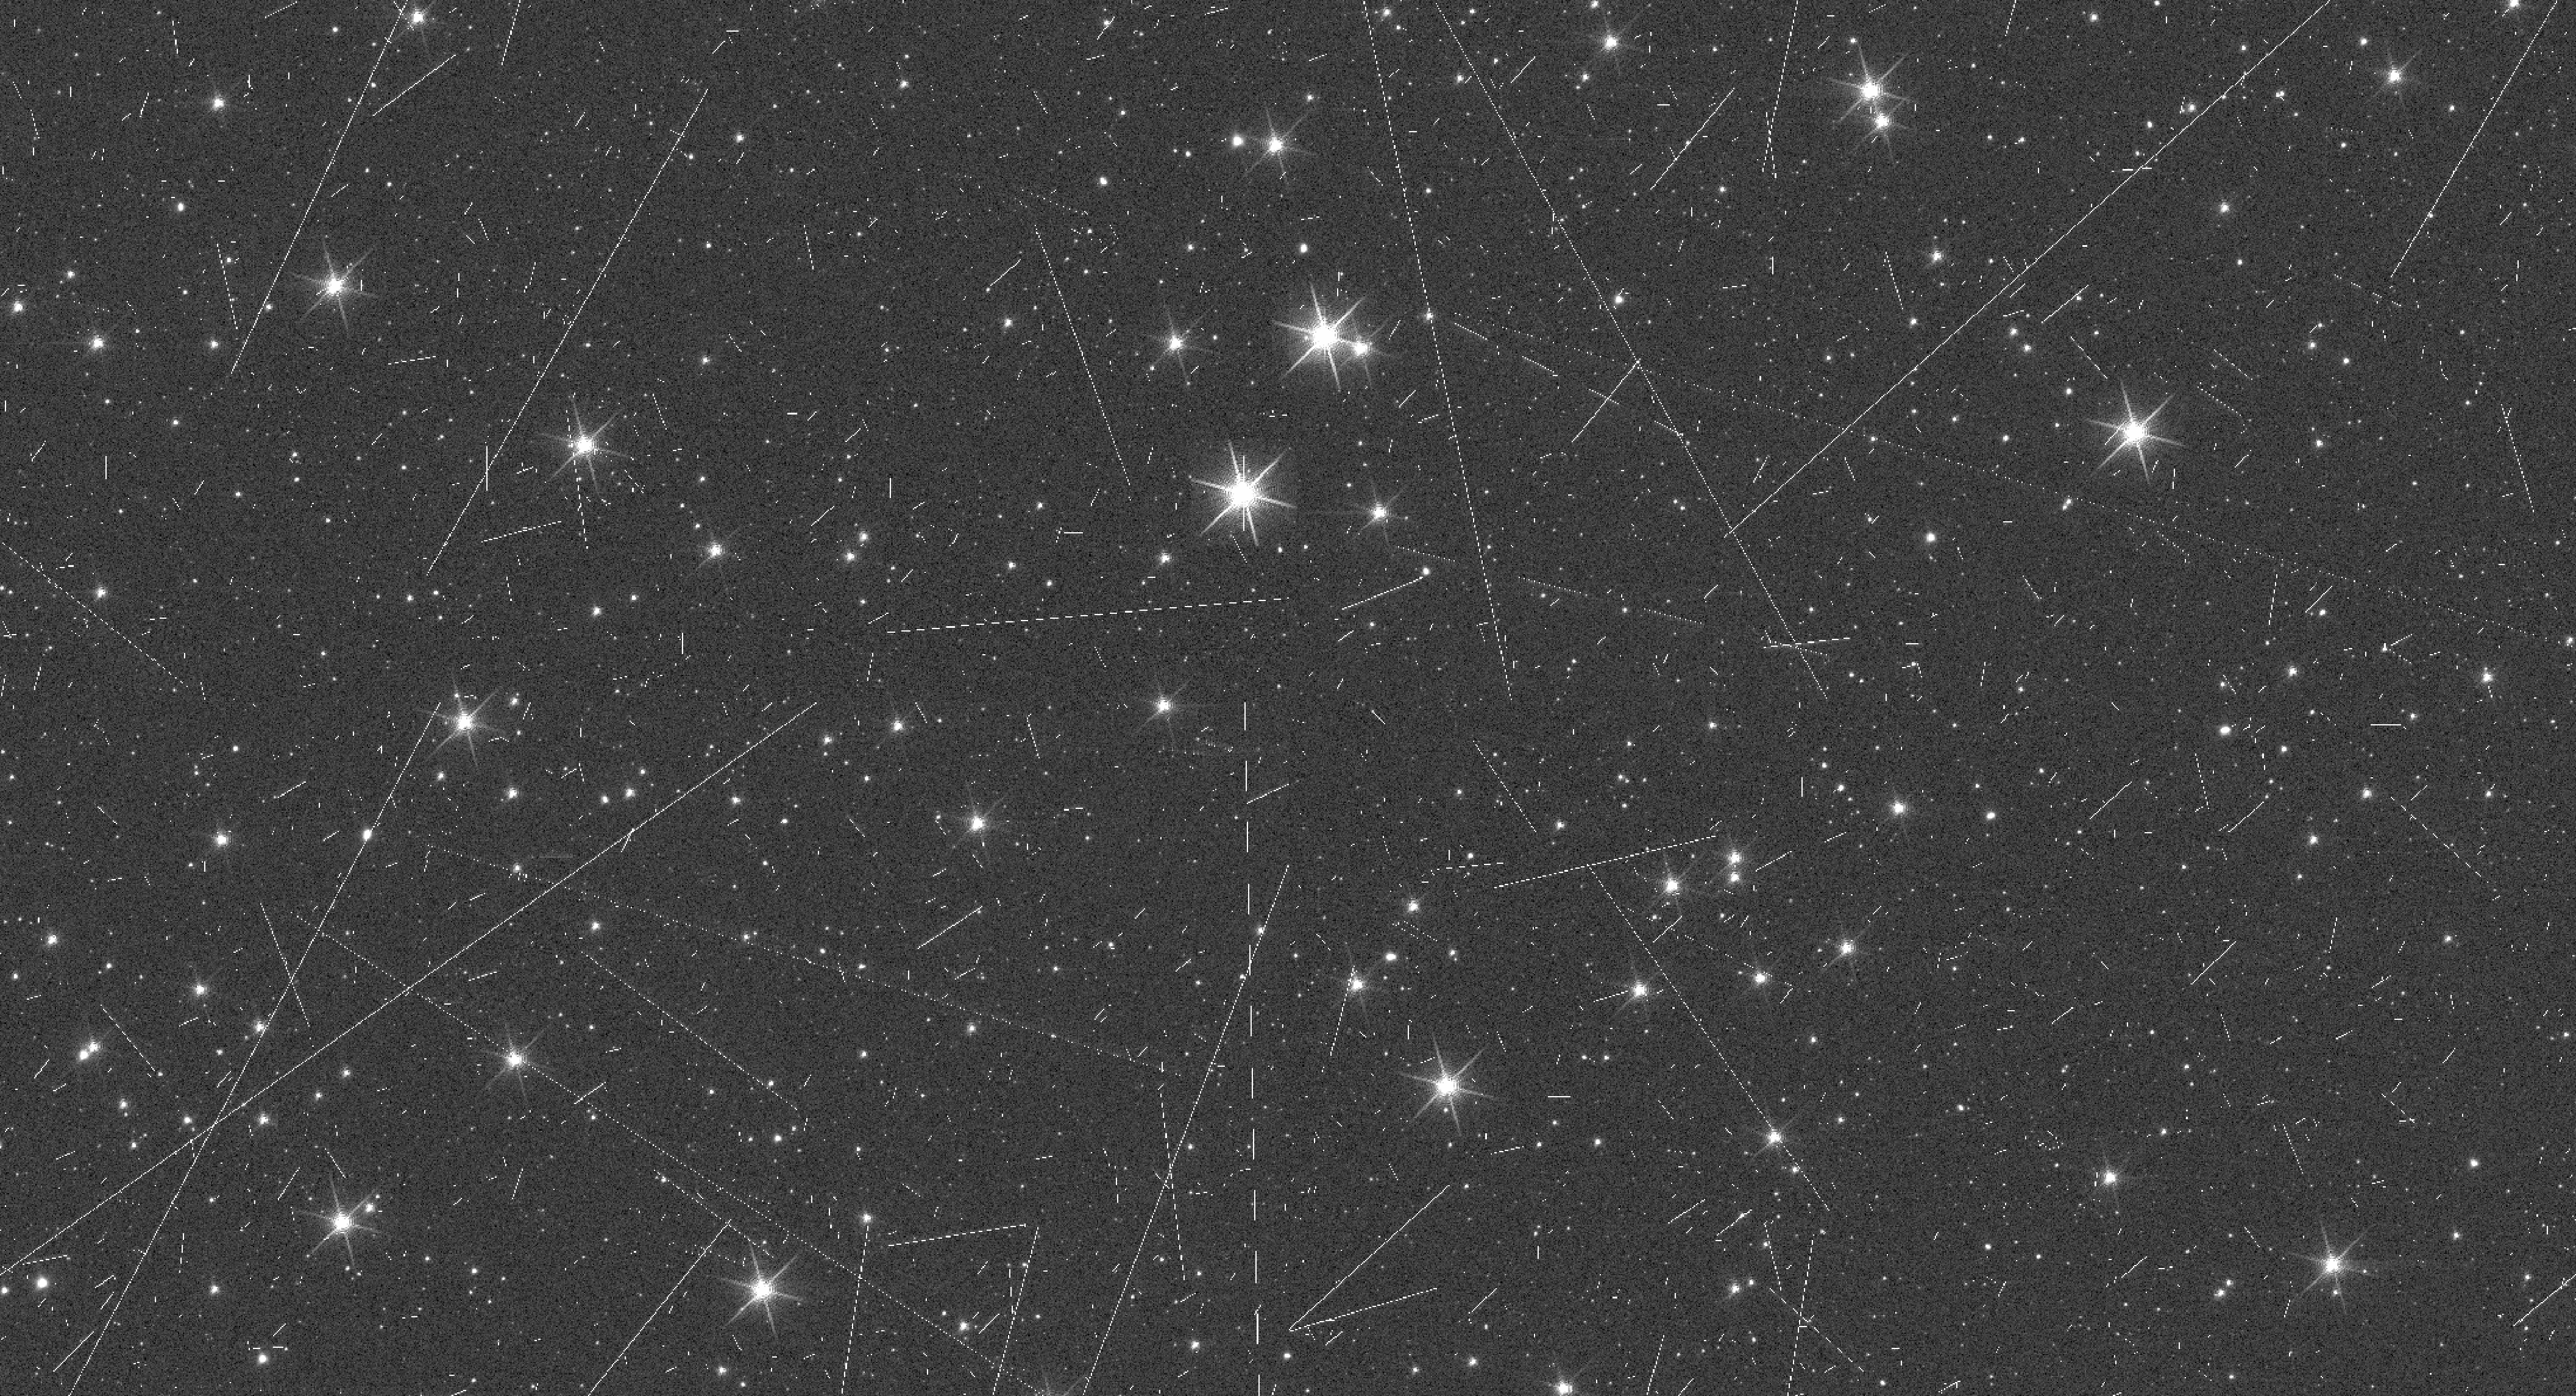
\includegraphics{simu.pdf}
\caption{An example image generated with the reference simulator. The image shows a part of a single
CCD.}\end{figure}


\chapter{Instrument Characteristics}
\label{index:instrument-characteristics}
The \emph{postproc} subpackage contains methods related to either generating a CCD mosaics from simulated data
that is in quadrants like the VIS reference simulator produces or including instrument characteristics
to simulated images that contain only Poisson noise and background. For more detailed documentation
of the Python classes, please see:


\section{Postprocessing tools}
\label{postproc:postprocessing-tools}\label{postproc::doc}\label{postproc:module-postproc.postprocessing}\index{postproc.postprocessing (module)}

\subsection{Inserting instrument characteristics}
\label{postproc:inserting-instrument-characteristics}
This file provides a class to insert instrument specific features to a simulated image. Supports multiprocessing.

\begin{notice}{note}{Note:}
The output images will be compressed with gzip to save disk space.
\end{notice}

\begin{notice}{warning}{Warning:}
The logging module used does not work well with multiprocessing, but
starts to write multiple entries after a while. This should be fixed.
\end{notice}
\begin{quote}\begin{description}
\item[{requires}] \leavevmode
PyFITS

\item[{requires}] \leavevmode
NumPy

\item[{requires}] \leavevmode
CDM03 (FORTRAN code, f2py -c -m cdm03 cdm03.f90)

\item[{author}] \leavevmode
Sami-Matias Niemi

\item[{contact}] \leavevmode
\href{mailto:smn2@mssl.ucl.ac.uk}{smn2@mssl.ucl.ac.uk}

\item[{version}] \leavevmode
0.8

\end{description}\end{quote}
\index{PostProcessing (class in postproc.postprocessing)}

\begin{fulllineitems}
\phantomsection\label{postproc:postproc.postprocessing.PostProcessing}\pysiglinewithargsret{\strong{class }\code{postproc.postprocessing.}\bfcode{PostProcessing}}{\emph{values}, \emph{work\_queue}, \emph{result\_queue}, \emph{seed}}{}
Euclid Visible Instrument postprocessing class. This class allows
to add radiation damage (as defined by the CDM03 model) and add
readout noise to a simulated image.
\index{applyLinearCorrection() (postproc.postprocessing.PostProcessing method)}

\begin{fulllineitems}
\phantomsection\label{postproc:postproc.postprocessing.PostProcessing.applyLinearCorrection}\pysiglinewithargsret{\bfcode{applyLinearCorrection}}{\emph{image}}{}
Applies a linear correction after one forward readout through the CDM03 model.

Bristow \& Alexov (2003) algorithm further developed for HST data
processing by Massey, Rhodes et al.
\begin{quote}\begin{description}
\item[{Parameters}] \leavevmode
\textbf{image} (\emph{ndarray}) -- radiation damaged image

\item[{Returns}] \leavevmode
corrected image after single forward readout

\item[{Return type}] \leavevmode
ndarray

\end{description}\end{quote}

\end{fulllineitems}

\index{applyRadiationDamage() (postproc.postprocessing.PostProcessing method)}

\begin{fulllineitems}
\phantomsection\label{postproc:postproc.postprocessing.PostProcessing.applyRadiationDamage}\pysiglinewithargsret{\bfcode{applyRadiationDamage}}{\emph{data}, \emph{iquadrant=0}}{}
Apply radian damage based on FORTRAN CDM03 model. The method assumes that
input data covers only a single quadrant defined by the iquadrant integer.
\begin{quote}\begin{description}
\item[{Parameters}] \leavevmode\begin{itemize}
\item {} 
\textbf{data} (\emph{ndarray}) -- imaging data to which the CDM03 model will be applied to.

\item {} 
\textbf{iquandrant} (\emph{int}) -- number of the quadrant to process

\end{itemize}

\end{description}\end{quote}
\begin{description}
\item[{cdm03 - Function signature:}] \leavevmode
sout = cdm03(sinp,iflip,jflip,dob,rdose,in\_nt,in\_sigma,in\_tr,{[}xdim,ydim,zdim{]})

\item[{Required arguments:}] \leavevmode
sinp : input rank-2 array(`f') with bounds (xdim,ydim)
iflip : input int
jflip : input int
dob : input float
rdose : input float
in\_nt : input rank-1 array(`d') with bounds (zdim)
in\_sigma : input rank-1 array(`d') with bounds (zdim)
in\_tr : input rank-1 array(`d') with bounds (zdim)

\item[{Optional arguments:}] \leavevmode
xdim := shape(sinp,0) input int
ydim := shape(sinp,1) input int
zdim := len(in\_nt) input int

\item[{Return objects:}] \leavevmode
sout : rank-2 array(`f') with bounds (xdim,ydim)

\end{description}

\begin{notice}{note}{Note:}
Because Python/NumPy arrays are different row/column based, one needs
to be extra careful here. NumPy.asfortranarray will be called to get
an array laid out in Fortran order in memory. Before returning the
array will be laid out in memory in C-style (row-major order).
\end{notice}
\begin{quote}\begin{description}
\item[{Returns}] \leavevmode
image that has been run through the CDM03 model

\item[{Return type}] \leavevmode
ndarray

\end{description}\end{quote}

\end{fulllineitems}

\index{applyReadoutNoise() (postproc.postprocessing.PostProcessing method)}

\begin{fulllineitems}
\phantomsection\label{postproc:postproc.postprocessing.PostProcessing.applyReadoutNoise}\pysiglinewithargsret{\bfcode{applyReadoutNoise}}{\emph{data}}{}
Applies readout noise. The noise is drawn from a Normal (Gaussian) distribution.
Mean = 0.0, and std = sqrt(readout).
\begin{quote}\begin{description}
\item[{Parameters}] \leavevmode
\textbf{data} (\emph{ndarray}) -- input data to which the readout noise will be added to

\item[{Returns}] \leavevmode
updated data, noise image

\item[{Return type}] \leavevmode
dict

\end{description}\end{quote}

\end{fulllineitems}

\index{compressAndRemoveFile() (postproc.postprocessing.PostProcessing method)}

\begin{fulllineitems}
\phantomsection\label{postproc:postproc.postprocessing.PostProcessing.compressAndRemoveFile}\pysiglinewithargsret{\bfcode{compressAndRemoveFile}}{\emph{filename}}{}
This method compresses the given file using gzip and removes the parent from
the file system.
\begin{quote}\begin{description}
\item[{Parameters}] \leavevmode
\textbf{filename} (\emph{str}) -- name of the file to be compressed

\item[{Returns}] \leavevmode
None

\end{description}\end{quote}

\end{fulllineitems}

\index{cutoutRegion() (postproc.postprocessing.PostProcessing method)}

\begin{fulllineitems}
\phantomsection\label{postproc:postproc.postprocessing.PostProcessing.cutoutRegion}\pysiglinewithargsret{\bfcode{cutoutRegion}}{\emph{data}}{}
Cuts out a region from the imaging data. The cutout region is specified by
xstart/stop and ystart/stop that are read out from the self.values dictionary.
Also checks if there are values that are above the given cutoff value and sets
those pixels to a max value (default=33e3).
\begin{quote}\begin{description}
\item[{Parameters}] \leavevmode\begin{itemize}
\item {} 
\textbf{data} (\emph{ndarray}) -- image array

\item {} 
\textbf{max} (\emph{int or float}) -- maximum allowed value {[}default = 33e3{]}

\end{itemize}

\item[{Returns}] \leavevmode
cut out image from the original data

\item[{Return type}] \leavevmode
ndarray

\end{description}\end{quote}

\end{fulllineitems}

\index{discretisetoADUs() (postproc.postprocessing.PostProcessing method)}

\begin{fulllineitems}
\phantomsection\label{postproc:postproc.postprocessing.PostProcessing.discretisetoADUs}\pysiglinewithargsret{\bfcode{discretisetoADUs}}{\emph{data}}{}
Convert floating point arrays to integer arrays and convert to ADUs.
Adds bias level after converting to ADUs.
\begin{quote}\begin{description}
\item[{Parameters}] \leavevmode
\textbf{data} (\emph{ndarray}) -- data to be discretised to.

\item[{Returns}] \leavevmode
discretised array in ADUs

\item[{Return type}] \leavevmode
ndarray

\end{description}\end{quote}

\end{fulllineitems}

\index{generateCTImap() (postproc.postprocessing.PostProcessing method)}

\begin{fulllineitems}
\phantomsection\label{postproc:postproc.postprocessing.PostProcessing.generateCTImap}\pysiglinewithargsret{\bfcode{generateCTImap}}{\emph{CTIed}, \emph{originalData}}{}
Calculates a map showing the CTI effect. This map is being
generated by dividing radiation damaged image with the original
data.
\begin{quote}\begin{description}
\item[{Parameters}] \leavevmode\begin{itemize}
\item {} 
\textbf{CTIed} (\emph{ndarray}) -- Radiation damaged image

\item {} 
\textbf{originalData} (\emph{ndarray}) -- Original image before any radiation damage

\end{itemize}

\item[{Returns}] \leavevmode
CTI map (ratio of radiation damaged image and original data)

\item[{Return type}] \leavevmode
ndarray

\end{description}\end{quote}

\end{fulllineitems}

\index{loadFITS() (postproc.postprocessing.PostProcessing method)}

\begin{fulllineitems}
\phantomsection\label{postproc:postproc.postprocessing.PostProcessing.loadFITS}\pysiglinewithargsret{\bfcode{loadFITS}}{\emph{filename}, \emph{ext=0}}{}
Loads data from a given FITS file and extension.
\begin{quote}\begin{description}
\item[{Parameters}] \leavevmode\begin{itemize}
\item {} 
\textbf{filename} (\emph{str}) -- name of the FITS file

\item {} 
\textbf{ext} (\emph{int}) -- FITS header extension {[}default=0{]}

\end{itemize}

\item[{Returns}] \leavevmode
data, FITS header, xsize, ysize

\item[{Return type}] \leavevmode
dict

\end{description}\end{quote}

\end{fulllineitems}

\index{radiateFullCCD() (postproc.postprocessing.PostProcessing method)}

\begin{fulllineitems}
\phantomsection\label{postproc:postproc.postprocessing.PostProcessing.radiateFullCCD}\pysiglinewithargsret{\bfcode{radiateFullCCD}}{\emph{fullCCD}, \emph{quads=(0}, \emph{1}, \emph{2}, \emph{3)}, \emph{xsize=2048}, \emph{ysize=2066}}{}
This routine allows the whole CCD to be run through a radiation damage mode.
The routine takes into account the fact that the amplifiers are in the corners
of the CCD. The routine assumes that the CCD is using four amplifiers.
\begin{quote}\begin{description}
\item[{Parameters}] \leavevmode\begin{itemize}
\item {} 
\textbf{fullCCD} (\emph{ndarray}) -- image of containing the whole CCD

\item {} 
\textbf{quads} (\emph{list}) -- quadrants, numbered from lower left

\end{itemize}

\item[{Returns}] \leavevmode
radiation damaged image

\item[{Return type}] \leavevmode
ndarray

\end{description}\end{quote}

\end{fulllineitems}

\index{run() (postproc.postprocessing.PostProcessing method)}

\begin{fulllineitems}
\phantomsection\label{postproc:postproc.postprocessing.PostProcessing.run}\pysiglinewithargsret{\bfcode{run}}{}{}
This is the method that will be called when multiprocessing.

\end{fulllineitems}

\index{writeFITSfile() (postproc.postprocessing.PostProcessing method)}

\begin{fulllineitems}
\phantomsection\label{postproc:postproc.postprocessing.PostProcessing.writeFITSfile}\pysiglinewithargsret{\bfcode{writeFITSfile}}{\emph{data}, \emph{output}, \emph{unsigned16bit=True}}{}
Write out FITS files using PyFITS.
\begin{quote}\begin{description}
\item[{Parameters}] \leavevmode\begin{itemize}
\item {} 
\textbf{data} (\emph{ndarray}) -- data to write to a FITS file

\item {} 
\textbf{output} (\emph{string}) -- name of the output file

\item {} 
\textbf{unsigned16bit} (\emph{bool}) -- whether to scale the data using bzero=32768

\end{itemize}

\item[{Returns}] \leavevmode
None

\end{description}\end{quote}

\end{fulllineitems}


\end{fulllineitems}

\phantomsection\label{postproc:module-postproc.tileCCD}\index{postproc.tileCCD (module)}

\subsection{Generating a mosaic}
\label{postproc:generating-a-mosaic}
This file contains a class to create a single VIS CCD image from separate files one for each quadrant.
\begin{quote}\begin{description}
\item[{requires}] \leavevmode
NumPy

\item[{requires}] \leavevmode
PyFITS

\item[{author}] \leavevmode
Sami-Matias Niemi

\item[{contact}] \leavevmode
\href{mailto:smn2@mssl.ucl.ac.uk}{smn2@mssl.ucl.ac.uk}

\end{description}\end{quote}

To execute:

\begin{Verbatim}[commandchars=\\\{\}]
python tileCCD.py -f 'Q*science.fits' -e 1
\end{Verbatim}

where -f argument defines the input files to be tiled and the -e argument marks the
FITS extension from which the imaging data are being read.
\begin{quote}\begin{description}
\item[{version}] \leavevmode
0.4

\end{description}\end{quote}
\index{tileCCD (class in postproc.tileCCD)}

\begin{fulllineitems}
\phantomsection\label{postproc:postproc.tileCCD.tileCCD}\pysiglinewithargsret{\strong{class }\code{postproc.tileCCD.}\bfcode{tileCCD}}{\emph{inputs}, \emph{log}}{}
Class to create a single VIS CCD image from separate quadrants files.
\index{readData() (postproc.tileCCD.tileCCD method)}

\begin{fulllineitems}
\phantomsection\label{postproc:postproc.tileCCD.tileCCD.readData}\pysiglinewithargsret{\bfcode{readData}}{}{}
Reads in data from all the input files and the header from the first file.
Input files are taken from the input dictionary given when class was initiated.

Subtracts the pre- and overscan regions if these were simulated. Takes into account
which quadrant is being processed so that the extra regions are subtracted correctly.

\end{fulllineitems}

\index{runAll() (postproc.tileCCD.tileCCD method)}

\begin{fulllineitems}
\phantomsection\label{postproc:postproc.tileCCD.tileCCD.runAll}\pysiglinewithargsret{\bfcode{runAll}}{}{}
Wrapper to perform all class methods.

\end{fulllineitems}

\index{tileCCD() (postproc.tileCCD.tileCCD method)}

\begin{fulllineitems}
\phantomsection\label{postproc:postproc.tileCCD.tileCCD.tileCCD}\pysiglinewithargsret{\bfcode{tileCCD}}{\emph{xsize=2048}, \emph{ysize=2066}}{}
Tiles quadrants to form a single CCD image.

Assume that the input file naming convention is Qx\_CCDX\_CCDY\_name.fits.
\begin{quote}\begin{description}
\item[{Parameters}] \leavevmode\begin{itemize}
\item {} 
\textbf{xsize} (\emph{int}) -- length of a quadrant in column direction

\item {} 
\textbf{ysize} (\emph{int}) -- length of a quadrant in row direction

\end{itemize}

\item[{Returns}] \leavevmode
image array of size (ysize*2, xsize*2)

\item[{Return type}] \leavevmode
dnarray

\end{description}\end{quote}

\end{fulllineitems}

\index{writeFITSfile() (postproc.tileCCD.tileCCD method)}

\begin{fulllineitems}
\phantomsection\label{postproc:postproc.tileCCD.tileCCD.writeFITSfile}\pysiglinewithargsret{\bfcode{writeFITSfile}}{\emph{data=None}, \emph{unsigned16bit=True}}{}
Write out FITS files using PyFITS.
\begin{quote}\begin{description}
\item[{Parameters}] \leavevmode\begin{itemize}
\item {} 
\textbf{data} (\emph{ndarray}) -- data to write to a FITS file, if None use self.data

\item {} 
\textbf{unsigned16bit} (\emph{bool}) -- whether to scale the data using bzero=32768

\end{itemize}

\item[{Returns}] \leavevmode
None

\end{description}\end{quote}

\end{fulllineitems}


\end{fulllineitems}



\chapter{Data reduction}
\label{index:data-reduction}
The \emph{reduction} subpackage contains a simple script to reduce VIS data. For more detailed documentation
of the classes, please see:


\section{Data reduction tools}
\label{reduction:module-reduction.reduceVISdata}\label{reduction::doc}\label{reduction:data-reduction-tools}\index{reduction.reduceVISdata (module)}

\subsection{VIS Data Reduction and Processing}
\label{reduction:vis-data-reduction-and-processing}
This simple script can be used to reduce (simulated) VIS data.

Does the following steps:

\begin{Verbatim}[commandchars=\\\{\}]
1 Bias correction
2 Flat fielding
3 CTI correction (conversion to electrons and back to ADUs)
\end{Verbatim}

To Run:

\begin{Verbatim}[commandchars=\\\{\}]
python reduceVISdata.py -i VISCCD.fits -b superBiasVIS.fits -f SuperFlatField.fits
\end{Verbatim}
\begin{quote}\begin{description}
\item[{requires}] \leavevmode
PyFITS

\item[{requires}] \leavevmode
NumPy

\item[{requires}] \leavevmode
CDM03 (FORTRAN code, f2py -c -m cdm03 cdm03.f90)

\item[{author}] \leavevmode
Sami-Matias Niemi

\item[{contact}] \leavevmode
\href{mailto:smn2@mssl.ucl.ac.uk}{smn2@mssl.ucl.ac.uk}

\item[{version}] \leavevmode
0.4

\end{description}\end{quote}

\begin{notice}{note}{Todo}
\begin{enumerate}
\item {} 
FITS extension should probably be read from the command line

\item {} 
implement background/sky subtraction

\end{enumerate}
\end{notice}
\index{reduceVISdata (class in reduction.reduceVISdata)}

\begin{fulllineitems}
\phantomsection\label{reduction:reduction.reduceVISdata.reduceVISdata}\pysiglinewithargsret{\strong{class }\code{reduction.reduceVISdata.}\bfcode{reduceVISdata}}{\emph{values}, \emph{log}}{}
Simple class to reduce VIS data.
\index{applyCTICorrection() (reduction.reduceVISdata.reduceVISdata method)}

\begin{fulllineitems}
\phantomsection\label{reduction:reduction.reduceVISdata.reduceVISdata.applyCTICorrection}\pysiglinewithargsret{\bfcode{applyCTICorrection}}{}{}
Applies a CTI correction in electrons using CDM03 CTI model.
Converts the data to electrons using the gain value given in self.values.
The number of forward reads is defined by self.values{[}'order'{]} parameter.

Bristow \& Alexov (2003) algorithm further developed for HST data
processing by Massey, Rhodes et al.

There is probably an excess of .copy() calls here, but I had some problems
when calling the Fortran code so I added them for now.

\end{fulllineitems}

\index{flatfield() (reduction.reduceVISdata.reduceVISdata method)}

\begin{fulllineitems}
\phantomsection\label{reduction:reduction.reduceVISdata.reduceVISdata.flatfield}\pysiglinewithargsret{\bfcode{flatfield}}{}{}
Take into account pixel-to-pixel non-uniformity through multipicative flat fielding.

\end{fulllineitems}

\index{subtractBias() (reduction.reduceVISdata.reduceVISdata method)}

\begin{fulllineitems}
\phantomsection\label{reduction:reduction.reduceVISdata.reduceVISdata.subtractBias}\pysiglinewithargsret{\bfcode{subtractBias}}{}{}
Simply subtracts self.bias from the input data.

\end{fulllineitems}

\index{writeFITSfile() (reduction.reduceVISdata.reduceVISdata method)}

\begin{fulllineitems}
\phantomsection\label{reduction:reduction.reduceVISdata.reduceVISdata.writeFITSfile}\pysiglinewithargsret{\bfcode{writeFITSfile}}{}{}
Write out FITS files using PyFITS.

\end{fulllineitems}


\end{fulllineitems}



\chapter{Data Analysis}
\label{index:data-analysis}
The \emph{analysis} subpackage contains classes and scripts related to data analysis. A simple source finder and shape
measuring classes are provided together with a wrapper to analyse reduced VIS data. For more detailed
documentation of the classes, please see:


\section{VIS data analysis tools}
\label{analysis::doc}\label{analysis:module-analysis.analyse}\label{analysis:vis-data-analysis-tools}\index{analysis.analyse (module)}

\subsection{Object finding and measuring ellipticity}
\label{analysis:object-finding-and-measuring-ellipticity}
This script provides a class that can be used to analyse VIS data.
One can either choose to use a Python based source finding algorithm or
give a SExtractor catalog as an input. If an input catalog is provided
then the program assumes that X\_IMAGE and Y\_IMAGE columns are present
in the input file.
\begin{quote}\begin{description}
\item[{requires}] \leavevmode
PyFITS

\item[{requires}] \leavevmode
NumPy

\item[{requires}] \leavevmode
matplotlib

\item[{author}] \leavevmode
Sami-Matias Niemi

\item[{contact}] \leavevmode
\href{mailto:smn2@mssl.ucl.ac.uk}{smn2@mssl.ucl.ac.uk}

\item[{version}] \leavevmode
0.2

\end{description}\end{quote}
\index{analyseVISdata (class in analysis.analyse)}

\begin{fulllineitems}
\phantomsection\label{analysis:analysis.analyse.analyseVISdata}\pysiglinewithargsret{\strong{class }\code{analysis.analyse.}\bfcode{analyseVISdata}}{\emph{filename}, \emph{log}, \emph{**kwargs}}{}
Simple class that can be used to find objects and measure their ellipticities.

One can either choose to use a Python based source finding algorithm or
give a SExtractor catalog as an input. If an input catalog is provided
then the program assumes that X\_IMAGE and Y\_IMAGE columns are present
in the input file.
\begin{quote}\begin{description}
\item[{Parameters}] \leavevmode\begin{itemize}
\item {} 
\textbf{filename} (\emph{string}) -- name of the FITS file to be analysed.

\item {} 
\textbf{log} (\emph{instance}) -- logger

\item {} 
\textbf{kwargs} (\emph{dict}) -- additional keyword arguments

\end{itemize}

\end{description}\end{quote}

Settings dictionary contains all parameter values needed
for source finding and analysis.
\index{doAll() (analysis.analyse.analyseVISdata method)}

\begin{fulllineitems}
\phantomsection\label{analysis:analysis.analyse.analyseVISdata.doAll}\pysiglinewithargsret{\bfcode{doAll}}{}{}
Run all class methods sequentially.

\end{fulllineitems}

\index{findSources() (analysis.analyse.analyseVISdata method)}

\begin{fulllineitems}
\phantomsection\label{analysis:analysis.analyse.analyseVISdata.findSources}\pysiglinewithargsret{\bfcode{findSources}}{}{}
Finds sources from data that has been read in when the class was initiated.
Saves results such as x and y coordinates of the objects to self.sources.
x and y coordinates are also available directly in self.x and self.y.

\end{fulllineitems}

\index{measureEllipticity() (analysis.analyse.analyseVISdata method)}

\begin{fulllineitems}
\phantomsection\label{analysis:analysis.analyse.analyseVISdata.measureEllipticity}\pysiglinewithargsret{\bfcode{measureEllipticity}}{}{}
Measures ellipticity for all objects with coordinates (self.x, self.y).

Ellipticity is measured using Guassian weighted quadrupole moments.
See shape.py and especially the ShapeMeasurement class for more details.

\end{fulllineitems}

\index{plotEllipticityDistribution() (analysis.analyse.analyseVISdata method)}

\begin{fulllineitems}
\phantomsection\label{analysis:analysis.analyse.analyseVISdata.plotEllipticityDistribution}\pysiglinewithargsret{\bfcode{plotEllipticityDistribution}}{}{}
Creates a simple plot showing the derived ellipticity distribution.

\end{fulllineitems}

\index{readSources() (analysis.analyse.analyseVISdata method)}

\begin{fulllineitems}
\phantomsection\label{analysis:analysis.analyse.analyseVISdata.readSources}\pysiglinewithargsret{\bfcode{readSources}}{}{}
Reads in a list of sources from an external file. This method assumes
that the input source file is in SExtractor format. Input catalog is
saves to self.sources. x and y coordinates are also available directly in self.x and self.y.

\end{fulllineitems}

\index{writeResults() (analysis.analyse.analyseVISdata method)}

\begin{fulllineitems}
\phantomsection\label{analysis:analysis.analyse.analyseVISdata.writeResults}\pysiglinewithargsret{\bfcode{writeResults}}{}{}
Outputs results to an ascii file defined in self.settings. This ascii file
is in SExtractor format and contains the following columns:

\begin{Verbatim}[commandchars=\\\{\}]
1. X coordinate
2. Y coordinate
3. ellipticity
4. R\_\PYGZob{}2\PYGZcb{}
\end{Verbatim}

\end{fulllineitems}


\end{fulllineitems}

\phantomsection\label{analysis:module-analysis.shape}\index{analysis.shape (module)}

\subsection{Measuring a shape of an object}
\label{analysis:measuring-a-shape-of-an-object}
Simple class to measure quadrupole moments and ellipticity of an object.
\begin{quote}\begin{description}
\item[{requires}] \leavevmode
NumPy

\item[{requres}] \leavevmode
PyFITS

\item[{author}] \leavevmode
Sami-Matias Niemi

\item[{contact}] \leavevmode
\href{mailto:smn2@mssl.ucl.ac.uk}{smn2@mssl.ucl.ac.uk}

\item[{version}] \leavevmode
0.2

\end{description}\end{quote}
\index{shapeMeasurement (class in analysis.shape)}

\begin{fulllineitems}
\phantomsection\label{analysis:analysis.shape.shapeMeasurement}\pysiglinewithargsret{\strong{class }\code{analysis.shape.}\bfcode{shapeMeasurement}}{\emph{data}, \emph{log}, \emph{**kwargs}}{}
Provides methods to measure the shape of an object.
\begin{quote}\begin{description}
\item[{Parameters}] \leavevmode\begin{itemize}
\item {} 
\textbf{data} (\emph{ndarray}) -- name of the FITS file to be analysed.

\item {} 
\textbf{log} (\emph{instance}) -- logger

\item {} 
\textbf{kwargs} (\emph{dict}) -- additional keyword arguments

\end{itemize}

\end{description}\end{quote}

Settings dictionary contains all parameter values needed.
\index{circular2DGaussian() (analysis.shape.shapeMeasurement method)}

\begin{fulllineitems}
\phantomsection\label{analysis:analysis.shape.shapeMeasurement.circular2DGaussian}\pysiglinewithargsret{\bfcode{circular2DGaussian}}{\emph{x}, \emph{y}, \emph{sigma}}{}
Create a circular symmetric Gaussian centered on x, y.
\begin{quote}\begin{description}
\item[{Parameters}] \leavevmode\begin{itemize}
\item {} 
\textbf{x} (\emph{float}) -- x coordinate of the centre

\item {} 
\textbf{y} (\emph{float}) -- y coordinate of the centre

\item {} 
\textbf{sigma} (\emph{float}) -- standard deviation of the Gaussian, note that sigma\_x = sigma\_y = sigma

\end{itemize}

\item[{Returns}] \leavevmode
circular Gaussian 2D profile and x and y mesh grid

\item[{Return type}] \leavevmode
dict

\end{description}\end{quote}

\end{fulllineitems}

\index{measureRefinedEllipticity() (analysis.shape.shapeMeasurement method)}

\begin{fulllineitems}
\phantomsection\label{analysis:analysis.shape.shapeMeasurement.measureRefinedEllipticity}\pysiglinewithargsret{\bfcode{measureRefinedEllipticity}}{}{}
Derive a refined iterated ellipticity measurement for a given object.

By default ellipticity is defined in terms of the Gaussian weighted quadrupole moments.
If self.settings{[}'weigted'{]} is False then no weighting scheme is used.
The number of iterations is defined in self.settings{[}'iterations'{]}.

:return centroids, ellipticity (including projected e1 and e2), and R2
:rtype: dict

\end{fulllineitems}

\index{quadrupoles() (analysis.shape.shapeMeasurement method)}

\begin{fulllineitems}
\phantomsection\label{analysis:analysis.shape.shapeMeasurement.quadrupoles}\pysiglinewithargsret{\bfcode{quadrupoles}}{\emph{image}}{}
Derive quadrupole moments and ellipticity from the input image.
\begin{quote}\begin{description}
\item[{Parameters}] \leavevmode
\textbf{image} (\emph{ndarray}) -- input image data

\item[{Returns}] \leavevmode
quadrupoles, centroid, and ellipticity (also the projected components e1, e2)

\item[{Return type}] \leavevmode
dict

\end{description}\end{quote}

\end{fulllineitems}

\index{writeFITS() (analysis.shape.shapeMeasurement method)}

\begin{fulllineitems}
\phantomsection\label{analysis:analysis.shape.shapeMeasurement.writeFITS}\pysiglinewithargsret{\bfcode{writeFITS}}{\emph{data}, \emph{output}}{}
Write out a FITS file using PyFITS.
\begin{quote}\begin{description}
\item[{Parameters}] \leavevmode\begin{itemize}
\item {} 
\textbf{data} (\emph{ndarray}) -- data to write to a FITS file

\item {} 
\textbf{output} (\emph{string}) -- name of the output file

\end{itemize}

\item[{Returns}] \leavevmode
None

\end{description}\end{quote}

\end{fulllineitems}


\end{fulllineitems}

\phantomsection\label{analysis:module-analysis.sourceFinder}\index{analysis.sourceFinder (module)}

\subsection{Object finding}
\label{analysis:object-finding}
Simple source finder that can be used to find objects from astronomical images.
\begin{quote}\begin{description}
\item[{reqiures}] \leavevmode
NumPy

\item[{requires}] \leavevmode
SciPy

\item[{requires}] \leavevmode
matplotlib

\item[{author}] \leavevmode
Sami-Matias Niemi

\item[{contact}] \leavevmode
\href{mailto:smn2@mssl.ucl.ac.uk}{smn2@mssl.ucl.ac.uk}

\item[{version}] \leavevmode
0.2

\end{description}\end{quote}
\index{sourceFinder (class in analysis.sourceFinder)}

\begin{fulllineitems}
\phantomsection\label{analysis:analysis.sourceFinder.sourceFinder}\pysiglinewithargsret{\strong{class }\code{analysis.sourceFinder.}\bfcode{sourceFinder}}{\emph{image}, \emph{log}, \emph{**kwargs}}{}
This class provides methods for source finding.
\begin{quote}\begin{description}
\item[{Parameters}] \leavevmode\begin{itemize}
\item {} 
\textbf{image} (\emph{numpy.ndarray}) -- 2D image array

\item {} 
\textbf{log} (\emph{instance}) -- logger

\item {} 
\textbf{kwargs} (\emph{dictionary}) -- additional keyword arguments

\end{itemize}

\end{description}\end{quote}
\index{cleanSample() (analysis.sourceFinder.sourceFinder method)}

\begin{fulllineitems}
\phantomsection\label{analysis:analysis.sourceFinder.sourceFinder.cleanSample}\pysiglinewithargsret{\bfcode{cleanSample}}{}{}
Cleans up small connected components and large structures.

\end{fulllineitems}

\index{find() (analysis.sourceFinder.sourceFinder method)}

\begin{fulllineitems}
\phantomsection\label{analysis:analysis.sourceFinder.sourceFinder.find}\pysiglinewithargsret{\bfcode{find}}{}{}
Find all pixels above the median pixel after smoothing with a Gaussian filter.

\begin{notice}{note}{Note:}
maybe one should use mode instead of median?
\end{notice}

\end{fulllineitems}

\index{generateOutput() (analysis.sourceFinder.sourceFinder method)}

\begin{fulllineitems}
\phantomsection\label{analysis:analysis.sourceFinder.sourceFinder.generateOutput}\pysiglinewithargsret{\bfcode{generateOutput}}{}{}
Outputs the found positions to an ascii and a DS9 reg file.
\begin{quote}\begin{description}
\item[{Returns}] \leavevmode
None

\end{description}\end{quote}

\end{fulllineitems}

\index{getCenterOfMass() (analysis.sourceFinder.sourceFinder method)}

\begin{fulllineitems}
\phantomsection\label{analysis:analysis.sourceFinder.sourceFinder.getCenterOfMass}\pysiglinewithargsret{\bfcode{getCenterOfMass}}{}{}
Finds the center-of-mass for all objects using numpy.ndimage.center\_of\_mass method.

\begin{notice}{note}{Note:}
these positions are zero indexed!
\end{notice}
\begin{quote}\begin{description}
\item[{Returns}] \leavevmode
xposition, yposition, center-of-masses

\item[{Return type}] \leavevmode
list

\end{description}\end{quote}

\end{fulllineitems}

\index{getContours() (analysis.sourceFinder.sourceFinder method)}

\begin{fulllineitems}
\phantomsection\label{analysis:analysis.sourceFinder.sourceFinder.getContours}\pysiglinewithargsret{\bfcode{getContours}}{}{}
Derive contours using the diskStructure function.

\end{fulllineitems}

\index{getFluxes() (analysis.sourceFinder.sourceFinder method)}

\begin{fulllineitems}
\phantomsection\label{analysis:analysis.sourceFinder.sourceFinder.getFluxes}\pysiglinewithargsret{\bfcode{getFluxes}}{}{}
Derive fluxes or counts.

\end{fulllineitems}

\index{getSizes() (analysis.sourceFinder.sourceFinder method)}

\begin{fulllineitems}
\phantomsection\label{analysis:analysis.sourceFinder.sourceFinder.getSizes}\pysiglinewithargsret{\bfcode{getSizes}}{}{}
Derives sizes for each object.

\end{fulllineitems}

\index{plot() (analysis.sourceFinder.sourceFinder method)}

\begin{fulllineitems}
\phantomsection\label{analysis:analysis.sourceFinder.sourceFinder.plot}\pysiglinewithargsret{\bfcode{plot}}{}{}
Generates a diagnostic plot.
\begin{quote}\begin{description}
\item[{Returns}] \leavevmode
None

\end{description}\end{quote}

\end{fulllineitems}

\index{runAll() (analysis.sourceFinder.sourceFinder method)}

\begin{fulllineitems}
\phantomsection\label{analysis:analysis.sourceFinder.sourceFinder.runAll}\pysiglinewithargsret{\bfcode{runAll}}{}{}
Performs all steps of source finding at one go.
\begin{quote}\begin{description}
\item[{Returns}] \leavevmode
source finding results such as positions, sizes, fluxes, etc.

\item[{Return type}] \leavevmode
dictionary

\end{description}\end{quote}

\end{fulllineitems}


\end{fulllineitems}


The \emph{data} subfolder contains the supporting data, such as cosmic ray distributions, cosmetics maps,
flat fielding files, PSFs, and an example configuration file.


\chapter{Charge Transfer Inefficiency}
\label{index:charge-transfer-inefficiency}
The \emph{fitting} subpackage contains a simple script that can be used to fit trap species so that the
Charge Transfer Inefficiency (CTI) trails forming behind charge injection lines agree with measured data.


\section{Fortran code for CTI}
\label{index:fortran-code-for-cti}
The \emph{fortran} folder contains a CDM03 CTI model Fortran code. For speed the CDM03 model has been written in Fortran
because it contains several nested loops. One can use f2py to compile the code to a format that can be imported
from Python.


\chapter{Supporting methods and files}
\label{index:supporting-methods-and-files}

\section{Objects}
\label{index:objects}
A few postage stamps showing observed galaxies have been placed to the \emph{objects} directory. These FITS files
can be used for, e.g., testing the shape measurement code.


\section{Code}
\label{index:code}
The \emph{support} subpackage contains some support classes and methods related to generating log files and read in
data.


\chapter{Photometric Accuracy}
\label{index:photometric-accuracy}
The reference simulator code has been tested against photometric accuracy (without aperture correction). A
simulated image was generated with the reference simulator, sources were identified and photometry performed
using SExtractor, and finally the extracted magnitudes were compared against the input catalog. The following
figure shows that the photometric accuracy with realistic noise and the end-of-life radiation damage is
about 0.08 mag without aperture correction. Please note, however, that the derived magnitudes are based on a
single 565 second exposure. Because of this the faint galaxies have low signal-to-noise ratio and therefore
the derived magnitudes are inaccurate.
\begin{figure}[htbp]
\centering
\capstart

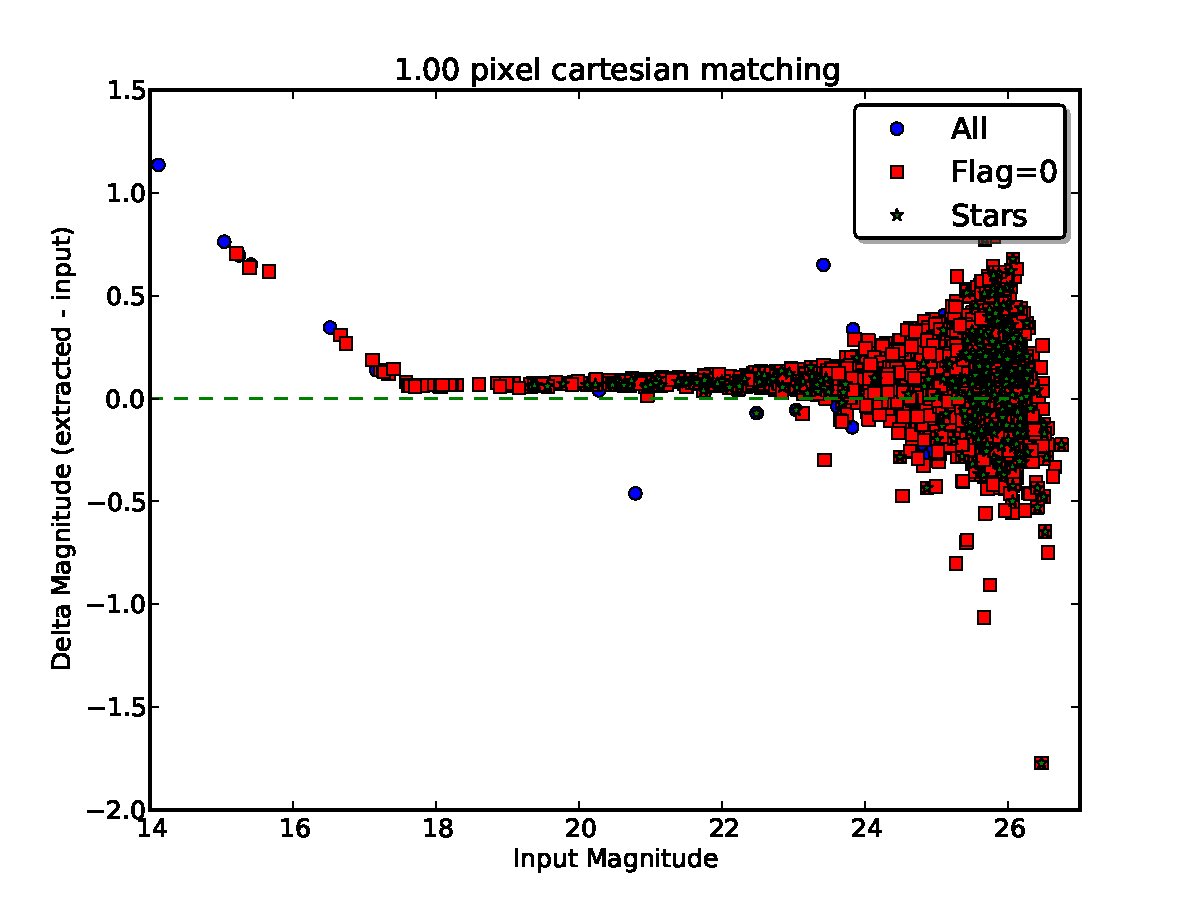
\includegraphics{Magnitudes15.pdf}
\caption{Example showing the recovered photometry from a reference simulator image with realistic noise
and end-of-life radiation damage, but without aperture correction. The offset is about 0.08mag.}\end{figure}


\chapter{Indices and tables}
\label{index:indices-and-tables}\begin{itemize}
\item {} 
\emph{genindex}

\item {} 
\emph{modindex}

\item {} 
\emph{search}

\end{itemize}


\renewcommand{\indexname}{Python Module Index}
\begin{theindex}
\def\bigletter#1{{\Large\sffamily#1}\nopagebreak\vspace{1mm}}
\bigletter{a}
\item {\texttt{analysis.analyse}}, \pageref{analysis:module-analysis.analyse}
\item {\texttt{analysis.shape}}, \pageref{analysis:module-analysis.shape}
\item {\texttt{analysis.sourceFinder}}, \pageref{analysis:module-analysis.sourceFinder}
\indexspace
\bigletter{p}
\item {\texttt{postproc.postprocessing}}, \pageref{postproc:module-postproc.postprocessing}
\item {\texttt{postproc.tileCCD}}, \pageref{postproc:module-postproc.tileCCD}
\indexspace
\bigletter{r}
\item {\texttt{reduction.reduceVISdata}}, \pageref{reduction:module-reduction.reduceVISdata}
\indexspace
\bigletter{s}
\item {\texttt{simulator.generateGalaxies}}, \pageref{simulator:module-simulator.generateGalaxies}
\item {\texttt{simulator.simulator}}, \pageref{simulator:module-simulator.simulator}
\item {\texttt{sources.createObjectCatalogue}}, \pageref{sources:module-sources.createObjectCatalogue}
\end{theindex}

\renewcommand{\indexname}{Index}
\printindex
\end{document}
